% SC2203 --- Chapter 7: Decidability and Undecidability (0->100 ground-up)
\chapter{Decidability, Undecidability and Reductions}
\label{ch:decidability}

\begin{quote}
\emph{``There are problems no algorithm can solve.''} --- Diagonalisation and reductions prove the halting problem undecidable, then transport that impossibility to every non-trivial property of programs via Rice's theorem.
\end{quote}

\noindent\fbox{\parbox{\dimexpr\linewidth-2\fboxsep-2\fboxrule}{%
\textbf{From zero: we build here, no undecidability assumed.} We define decidable vs.\ recognisable from Ch.~6 TMs, prove halting undecidable by diagonalisation, then build mapping reductions and Rice. Only TM definitions and encodings $\langle M,w\rangle$ required.}}
\vspace{0.4em}

\section*{Learning Outcomes}
After this chapter you will be able to:
\begin{enumerate}[label=(L\arabic*)]
    \item distinguish decidable (recursive), recognisable (r.e.) and co-recognisable;
    \item state and prove $HALT$ undecidable via diagonalisation;
    \item construct mapping reductions $A\le_m B$ and use them to transfer (un)decidability;
    \item state Rice's theorem and apply it to semantic properties ($L(M)=\emptyset$, regularity, etc.);
    \item classify $A_{TM},E_{TM},EQ_{TM}$ as undecidable/recognisable with reductions.
\end{enumerate}

% ============================================================
\section{Decidable vs.\ Recognisable}
\label{sec:decidable-def}
Recall from Ch.~6: $L$ is \emph{decidable} if some TM decider halts on \emph{all} $w$ and $w\in L\iff$ accept. $L$ is \emph{recognisable} (r.e.) if some TM $M$ halts-accepts exactly on $w\in L$ (may loop otherwise). Decidable $\Rightarrow$ recognisable; converse fails strictly.

\begin{definition}[Complements and co-r.e.]
$\overline{L}=\Sigma^*\setminus L$. $L$ is \emph{co-recognisable} if $\overline{L}$ is recognisable. $L$ decidable iff $L$ and $\overline{L}$ both recognisable (run both recognisers in parallel---dovetail---and one must halt).
\end{definition}

% TikZ 1: landscape of languages
\begin{figure}[h]
\centering
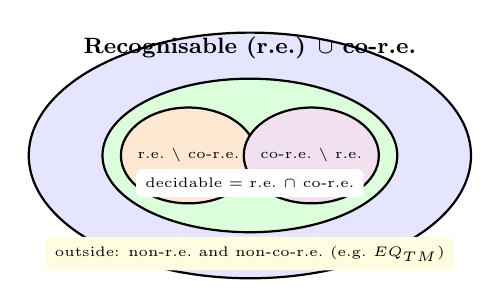
\begin{tikzpicture}[scale=0.78,every node/.style={font=\scriptsize}]
\draw[thick,fill=blue!10] (0,0) ellipse (3.6 and 2.0);
\draw[thick,fill=green!14] (0,0) ellipse (2.4 and 1.25);
\draw[thick,fill=orange!18] (-1.0,0) ellipse (1.1 and 0.78);
\draw[thick,fill=violet!12] (1.0,0) ellipse (1.1 and 0.78);
\node[font=\footnotesize\bfseries] at (0,1.75) {Recognisable (r.e.) $\cup$ co-r.e.};
\node[font=\tiny] at (-1.0,0) {r.e.\ $\setminus$ co-r.e.};
\node[font=\tiny] at (1.0,0) {co-r.e.\ $\setminus$ r.e.};
\node[font=\tiny,fill=white,rounded corners=2pt] at (0,-0.45) {decidable $=$ r.e.\ $\cap$ co-r.e.};
\node[font=\tiny,fill=yellow!12,rounded corners=2pt] at (0,-1.6) {outside: non-r.e.\ and non-co-r.e.\ (e.g.\ $EQ_{TM}$)};
\end{tikzpicture}
\caption{Decidable is the intersection of r.e.\ and co-r.e.; $HALT$ is r.e.\ but not decidable; $EQ_{TM}$ is neither. Diagonal languages live outside.}
\label{fig:decidable-landscape}
\end{figure}

\begin{example}[Decidable warm-ups]
$A_{DFA}=\{\langle D,w\rangle\mid D\text{ DFA accepts }w\}$ decidable (simulate DFA). $A_{CFG}=\{\langle G,w\rangle\mid G$ derives $w\}$ decidable (CYK). $E_{DFA}=\{\langle D\rangle\mid L(D)=\emptyset\}$ decidable (graph reachability). By contrast, $A_{TM}=\{\langle M,w\rangle\mid M$ accepts $w\}$ is recognisable (simulate $M$; accept if it does) but \emph{not} decidable---the gap starts with TMs.
\end{example}

\begin{remark}[Recognisable = enumerable]
We will use ``r.e.\ = recognisable = enumerable'' interchangeably. An enumerator is a TM that prints $L$'s strings (in any order, with repetitions allowed) without input; its existence is equivalent to a recogniser. Dovetailing gives the enumerator for recognisable $L$ explicitly.
\end{remark}

\begin{example}[Code: dovetail decider from two recognisers]
\begin{lstlisting}[language=Python]
def decider_for_L(w, M_L, M_comp):
    # M_L recognises L, M_comp recognises complement
    for t in range(1000000):  # dovetail by time bound t
        if simulates_accepts(M_L, w, t): return True
        if simulates_accepts(M_comp, w, t): return False
# Halts iff w in L or w not in L, i.e. iff both are r.e., yielding decidability
\end{lstlisting}
If both $L$ and $\overline{L}$ are r.e., this interleaving always halts, giving a decider; hence decidable = r.e.\ $\cap$ co-r.e.
\end{example}

% ============================================================
\section{The Halting Problem is Undecidable}
\label{sec:halting}
$HALT=\{\langle M,w\rangle\mid M\text{ halts on }w\}$; $A_{TM}$ is similar but requires \emph{acceptance}. HALT is r.e.\ (simulate, accept if halt) but undecidable.

\begin{theorem}[Turing, 1936 --- Halting undecidable]
$HALT$ (equivalently $A_{TM}$) is undecidable: no TM decider $H$ exists with $H(\langle M,w\rangle)=$ accept iff $M$ halts on $w$.
\end{theorem}
\begin{proof}[Diagonalisation]
Assume decider $H$ for HALT. Build $D$ on input $\langle M\rangle$: run $H(\langle M,\langle M\rangle\rangle)$; if $H$ says ``halts'' then $D$ loops forever (e.g.\ $\texttt{while True: pass}$), else $D$ halts. So $D(\langle M\rangle)$ halts iff $M(\langle M\rangle)$ loops. Now run $D$ on $\langle D\rangle$: $D(\langle D\rangle)$ halts iff $D(\langle D\rangle)$ loops---contradiction. Hence $H$ cannot exist. For $A_{TM}$, similar but $D$ rejects vs.\ accepts. \qed
\end{proof}

% TikZ 2: diagonal table
\begin{figure}[h]
\centering
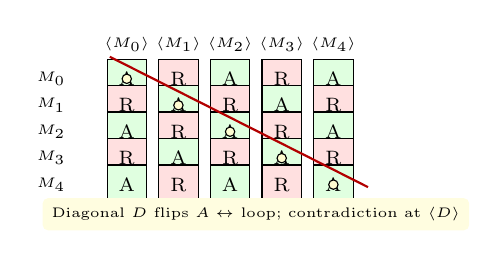
\begin{tikzpicture}[scale=0.80,every node/.style={font=\scriptsize}]
\foreach \i in {0,...,4} {\node[font=\tiny] at (-0.85,1.6-0.42*\i) {$M_{\i}$};}
\foreach \j in {0,...,4} {\node[font=\tiny] at (0.35+0.82*\j,2.15) {$\langle M_{\j}\rangle$};}
\foreach \i in {0,...,4} {\foreach \j in {0,...,4} {\pgfmathsetmacro{\x}{0.35+0.82*\j}\pgfmathsetmacro{\y}{1.6-0.42*\i}\pgfmathtruncatemacro{\v}{mod(\i+\j,2)}\ifnum\v=0 \node[fill=green!12,draw,minimum size=0.5cm] at (\x,\y) {A};\else \node[fill=red!12,draw,minimum size=0.5cm] at (\x,\y) {R};\fi}}
\draw[thick,red!70!black] (0.08,1.95)--(4.18,-0.12);
\foreach \i in {0,...,4} {\pgfmathsetmacro{\x}{0.35+0.82*\i}\pgfmathsetmacro{\y}{1.6-0.42*\i}\node[fill=yellow!18,draw,circle,inner sep=1.2pt] at (\x,\y) {};}
\node[font=\tiny,fill=yellow!12,rounded corners=2pt] at (2.4,-0.55) {Diagonal $D$ flips $A\leftrightarrow$ loop; contradiction at $\langle D\rangle$};
\end{tikzpicture}
\caption{Diagonal table: row $i$ is $M_i$'s behaviour on $\langle M_j\rangle$; $D$ flips the diagonal, so $D$ differs from every $M_i$---no decider for HALT can exist.}
\label{fig:diagonal}
\end{figure}

\begin{corollary}
$HALT$ is recognisable but not decidable; $\overline{HALT}$ is not recognisable. Hence decidability $\subsetneq$ recognisability.
\end{corollary}
The diagonalisation shows HALT's complement cannot be enumerated: no TM even lists all non-halting pairs. This is stronger than ``no decider''---it separates r.e.\ from co-r.e.

% ============================================================
\section{Mapping Reductions}
\label{sec:reductions}
Reductions transfer undecidability: ``if I could decide $B$, I could decide $A$''.

\begin{definition}[Mapping reduction]
$A\le_m B$ (reducible) if there is computable $f:\Sigma^*\to\Sigma^*$ with $w\in A\iff f(w)\in B$. $f$ is total computable (always halts) by a TM. If $A\le_m B$ and $B$ decidable then $A$ decidable (compose $f$ with decider for $B$); contrapositive: $A$ undecidable $\Rightarrow$ $B$ undecidable. Similarly for recognisability: $B$ r.e.\ $\Rightarrow$ $A$ r.e.
\end{definition}

% TikZ 3: reduction as computable map
\begin{figure}[h]
\centering
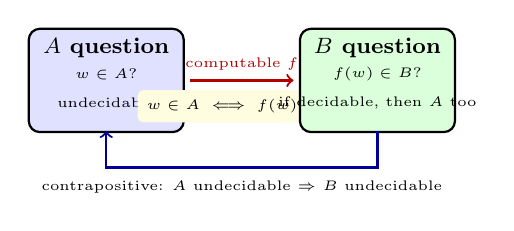
\begin{tikzpicture}[scale=0.82,every node/.style={font=\scriptsize}]
\draw[thick,fill=blue!12,rounded corners=4pt] (0,0) rectangle (2.4,1.6);
\node[font=\footnotesize\bfseries] at (1.2,1.3) {$A$ question};
\node[font=\tiny] at (1.2,0.9) {$w\in A?$};
\node[font=\tiny] at (1.2,0.45) {undecidable};
\draw[->,thick,red!70!black] (2.5,0.8)--(4.1,0.8) node[midway,above,font=\tiny] {computable $f$};
\node[font=\tiny,fill=yellow!12,rounded corners=2pt] at (3.3,0.4) {$w\in A\iff f(w)\in B$};
\draw[thick,fill=green!14,rounded corners=4pt] (4.2,0) rectangle (6.6,1.6);
\node[font=\footnotesize\bfseries] at (5.4,1.3) {$B$ question};
\node[font=\tiny] at (5.4,0.9) {$f(w)\in B?$};
\node[font=\tiny] at (5.4,0.45) {if decidable, then $A$ too};
\draw[->,thick,blue!60!black] (5.4,0.02)--(5.4,-0.55)--(1.2,-0.55)--(1.2,0.02);
\node[font=\tiny] at (3.3,-0.85) {contrapositive: $A$ undecidable $\Rightarrow$ $B$ undecidable};
\end{tikzpicture}
\caption{Mapping reduction: computable $f$ maps instances of $A$ to instances of $B$ preserving membership; decidability flows forward, undecidability flows backward.}
\label{fig:mapping-reduction}
\end{figure}

\begin{example}[HALT $\le_m$ $E_{TM}$? No, but $A_{TM}\le_m\overline{E_{TM}}$]
$E_{TM}=\{\langle M\rangle\mid L(M)=\emptyset\}$ is undecidable. Reduction from $A_{TM}$: given $\langle M,w\rangle$, build $M'$ that on $x$: if $x\neq w$ reject, else simulate $M$ on $w$ and accept iff $M$ accepts. Then $L(M')=\{w\}$ if $M$ accepts $w$, else $\emptyset$. So $\langle M,w\rangle\in A_{TM}\iff\langle M'\rangle\notin E_{TM}$. Hence $A_{TM}\le_m\overline{E_{TM}}$; since $A_{TM}$ undecidable and r.e., $\overline{E_{TM}}$ is r.e.\ but $E_{TM}$ is co-r.e.\ complete, neither decidable.
\end{example}

\begin{example}[Code: builder for $E_{TM}$ reduction]
\begin{lstlisting}[language=Python]
def f_A_to_notE(code_M, w):
    # return code of M' that isolates w
    def M_prime(x):
        if x != w: return False
        return simulate(M_code=code_M, input=w)  # accept iff M accepts w
    return encode(M_prime)
# Then w in A_TM iff f(w) not in E_TM
\end{lstlisting}
The builder is computable: we output the source code of $M'$ syntactically, not by running $M$.
\end{example}

% ============================================================
\section{Rice's Theorem: Every Non-Trivial Semantic Property is Undecidable}
\label{sec:rice}
A \emph{semantic} property depends only on $L(M)$, not on code shape or step count. Non-trivial = some TMs have it, some don't.

\begin{theorem}[Rice, 1953]
Let $\mathcal{P}\subseteq\mathcal{P}(\Sigma^*)$ be a set of languages. $L_{\mathcal{P}}=\{\langle M\rangle\mid L(M)\in\mathcal{P}\}$ is decidable iff $\mathcal{P}$ is trivial ($\emptyset$ or all r.e.\ languages). In particular, any non-trivial semantic property of $L(M)$ is undecidable.
\end{theorem}
\begin{proof}[Sketch]
Assume non-trivial, $\emptyset\notin\mathcal{P}$ w.l.o.g.\ (otherwise complement). Pick $M_0$ with $L(M_0)\in\mathcal{P}$. Reduction from $A_{TM}$: given $\langle M,w\rangle$, build $M'$ that on $x$: simulate $M$ on $w$ (without touching $x$); if $M$ accepts $w$, then run $M_0$ on $x$ and accept iff $M_0$ does. If $M$ never accepts, $M'$ loops forever on all $x$, so $L(M')=\emptyset\notin\mathcal{P}$; if $M$ accepts, $L(M')=L(M_0)\in\mathcal{P}$. Hence $\langle M,w\rangle\in A_{TM}\iff\langle M'\rangle\in L_{\mathcal{P}}$, so $A_{TM}\le_m L_{\mathcal{P}}$ and $L_{\mathcal{P}}$ undecidable. \qed
\end{proof}

\begin{example}[Rice in action]
``$L(M)$ is regular'', ``$L(M)$ finite'', ``$M$ halts on $\varepsilon$'', ``$L(M)=\Sigma^*$'' are all undecidable (non-trivial semantic). By contrast, ``$M$ has $5$ states'' is \emph{decidable} (syntactic, inspect code)---Rice does not apply.
\end{example}

% ============================================================
\section{Catalogue: $E_{TM},EQ_{TM},REG_{TM}$}
\label{sec:catalogue}
We classify canonical problems:
\begin{itemize}[leftmargin=1.2em]
    \item $A_{TM}$ r.e.\ but not decidable (as HALT).
    \item $E_{TM}=\{\langle M\rangle\mid L(M)=\emptyset\}$ co-r.e.\ but not r.e.\ (complement is r.e.\ via $A_{TM}\le_m\overline{E_{TM}}$); hence undecidable.
    \item $EQ_{TM}=\{\langle M_1,M_2\rangle\mid L(M_1)=L(M_2)\}$ neither r.e.\ nor co-r.e.\ (needs both).
    \item $REG_{TM}=\{\langle M\rangle\mid L(M)\text{ regular}\}$ undecidable by Rice, and neither r.e.\ nor co-r.e.
    \item $\overline{A_{TM}}$ not r.e.; dovetail shows decidable = r.e.\ $\cap$ co-r.e.
\end{itemize}
The picture in Fig.~\ref{fig:decidable-landscape} locates each; reductions justify the inclusions.

\subsection{Dovetailing: enumerating r.e.\ languages}
If $L$ r.e.\ via $M$, the strings in $L$ can be \emph{enumerated} by dovetailing: stage $t$ simulates $M$ on first $t$ strings for $t$ steps each, outputting those that accept within $t$. This enumerator lists $L$ without repetition; conversely an enumerator gives a recogniser. Dovetailing is the algorithmic picture of ``interleaving infinitely many simulations'' that makes decidable = r.e.\ $\cap$ co-r.e.\ constructive.

% ============================================================
\section{Chapter Notes}
G\"odel's incompleteness and Turing's halting are twin diagonalisations. Post and Kleene classified r.e.\ degrees; Rice's theorem (1953) subsumes countless undecidability proofs in one shot. For practice, always try Rice first for semantic $L(M)$ properties; if syntactic (states, transitions), Rice does not apply.
Mapping reductions $\le_m$ are many-one; stronger Turing reductions ($\le_T$) allow adaptive queries but are not needed for Rice. The arithmetical hierarchy ($\Sigma_1=$ r.e., $\Pi_1=$ co-r.e., $\Delta_1=$ decidable) organises these classes; $EQ_{TM}$ is $\Pi_2$-complete.

% ============================================================
\section{Exercises}
\label{sec:ch07-exercises}
Rice gives one-line undecidability for semantic properties; mapping reductions handle syntactic or mixed properties and completeness arguments.
For converse, recall: if $A\le_m B$ and $B$ r.e.\ then $A$ r.e.; contrapositive: $A$ not r.e.\ $\Rightarrow$ $B$ not r.e.\ (used for $EQ_{TM}$).
E7.4--E7.5 together show the decidable $\subsetneq$ r.e.\ hierarchy has at least four distinct levels.
% Strategy: to show $L$ not r.e., reduce $\overline{A_{TM}}$ (known non-r.e.) to $L$; to show $L$ not co-r.e., reduce $A_{TM}$ to $\overline{L}$.
\begin{enumerate}[label=E7.\arabic*, leftmargin=*, itemsep=0.8em]
\item \textbf{Diagonal warm-up.} Reprove $HALT$ undecidable by assuming $H$ decides it and deriving contradiction with $D(\langle D\rangle)$; explain why $D$ must loop (not just reject) to foil deciders that may expect reject vs.\ loop.
\item \textbf{Mapping reduction: $HALT\le_m E_{TM}$?} Give $f$ that maps $\langle M,w\rangle$ to $\langle M'\rangle$ with $L(M')=\emptyset$ iff $M$ does not halt? Correct the common mistake: halting vs.\ acceptance matters; produce $f$ for $A_{TM}\le_m\overline{E_{TM}}$ explicitly.
\item \textbf{Rice application.} Use Rice to prove $L=\{\langle M\rangle\mid |L(M)|\ge3\}$ undecidable, and $L'=\{\langle M\rangle\mid M\text{ has }10\text{ states}\}$ decidable; explain why Rice applies to $L$ but not $L'$.
\item \textbf{Co-r.e.\ complete.} Show $\overline{A_{TM}}$ is not r.e.: assume it were, then both $A_{TM}$ and $\overline{A_{TM}}$ r.e.\ would make $A_{TM}$ decidable---contradiction. Deduce $E_{TM}$ co-r.e.\ via complement reduction.
\item \textbf{Neither r.e.\ nor co-r.e.} Prove $EQ_{TM}$ neither r.e.\ nor co-r.e.: reduce $A_{TM}$ to $\overline{EQ}$ and $\overline{A_{TM}}$ to $EQ$ via suitable $f$ that builds $M_1,M_2$ with $L(M_1)=L(M_2)$ conditioned on halting.
\end{enumerate}
% End of Chapter 7
